\chapter{Peano's block-structured output format}


Peano has introduced its own block-structured output format.
Its idea is that a mesh is dumped as an unstructured set of cell where each cell
is uniquely identified through its offset and its size. 
The mesh data format lacks any topological information (connectivity).
A cell always is a patch, i.e.~holds a (topological) Cartesian mesh of
dimensions $k \times k$ or $k \times k \times k $, respectively.
If you work without patches, $k=2$. 
In this case, the block format obviously can yield a significant overhead.



\section{A minimal ASCII example file}
\begin{code}
#
# Peano output file
# Version 0.1
#
format ascii
dimensions 3
patch-size 6 6 6

begin vertex-values "identifier A"
  number-of-unknowns 58
  meta-data "This is some fancy meta data"  
end vertex-values

begin vertex-values "time"
  number-of-unknowns 1
  meta-data "This is some fancy meta data"  
end vertex-values

begin patch
  offset 0.0 0.0 0.0
  size   0.5 0.5 0.5
  begin vertex-values "identifier A"
    18.0 123.0 ...
  end vertex-values
  begin vertex-values "time"
    1.0 1.0 ...
  end vertex-values
end patch 

begin patch
  offset 0.5 0.0 0.0
  size   0.25 0.25 0.25
  ...
end patch 
\end{code}

\noindent
This spec file specifies a simple grid that

\begin{itemize}
  \item The actual grid plotted consists of two patches (boxes discretised with
  a small regular grid).
  \item Both small grids consist of $6 \times 6 \times 6$ cells. They all have
  the same size, i.e.~are equally spaced. 
  \item Each vertex holds two sets of unknowns. The first set is called
  \texttt{identifier A} and each entry (per vertex) comprises 58 double
  unknowns. The second set of unknowns per vertex is called \texttt{time} and is
  a scalar quantity.
  \item The data per cube is ordered lexicographically, i.e.~we run along the
  x-axis first, then along the y-axis, and finally along the z-axis. 
  \item All data is held as SoA, i.e.~we first give all the 58 unknowns of the
  first vertex within the cube, then the 58 unknowns of the right neighbour
  vertex, and so forth.
  \item All output data is ASCII.
  \item Patches may overlap in both space and time.
\end{itemize}


\noindent
If you use Peano's HDF5 file format, please note that you typically obtain
a bunch of files. 
A meta file whose name coincides with the one you specify in your specification
file. 
This meta file contains links to the actual data files. 
Its syntax is self-explaining and you can open it with a plain text editor.


\section{More sophiciated dumps}

\begin{itemize}
  \item The file format supports \texttt{cell-values}.
%   \item In our example, we stick to ASCII data. The file format however also
%   supports \texttt{binary} data in which case everything within
%   \texttt{vertex-values} and \texttt{cell-values} is dumped as binary stream.
%   Finally, we plan to provide \texttt{hdf5} data dumps in which case only one
%   integer is stored within the \texttt{vertex-values} or \texttt{cell-values}
%   sections which identifies the row in the hdf5 data dump.
%   \item Other data file fragments can be included via \texttt{include}
%   statements.
  \item Each \texttt{vertex-values} or \texttt{cell-values} section in the
  header of the file, i.e.~not embedded into a patch, may have a section
  \begin{code}
   begin mapping
     0.0 0.0 0.0
     0.1 0.1 0.1
     0.4 0.4 0.4
     ...
   end mapping
  \end{code} 
  If no mapping is present, our code dumps a regular subgrid (patch) per
  \texttt{patch} region. If a mapping is present, the mapping has exactly $(6+1)
  \cdot (6+1) \cdot (6+1)$ entries in the example from the previous section.
  Each entry is a 3d coordinate relative to the unit cube and specifies how the
  topologially regular grid prescribed within a patch is to be mapped. You might
  for example plot points of the topologically regular grid with 
  Gau\ss -Legendre spacing.
  \item The plotter by default always creates two types of files: The actual
  data files as described above and one meta file. The meta file solely links to
  the actual data:
  \begin{code}
# 
# Peano patch file 
# Version 0.1 
# 
format ASCII
begin dataset
  include "conserved-1-rank-0.peano-patch-file"
end dataset
begin dataset
  include "conserved-2-rank-0.peano-patch-file"
end dataset
  \end{code}
  Per snapshot (typically time step), the plotter adds on \texttt{dataset}
  entry. Each data set holds one data file per active rank. Each rank writes its
  actual data into a separate file. 
\end{itemize}


\section{Convert into VTK}

Peano ships some C++ visualisation scripts which can convert the patch file
format into plain VTK.
To use them, you have to translate Peano with VTK support (cmp.~configure
script in \ref{section:installation:configure}).
The script can be found in the \texttt{visualisation} subdirectory of
\texttt{src} and provides extensive usage instructions if you invoke it without
arguments.

% \section{Peano's HDF5 format}
% 
% The lack of connectivity data renders the streaming into HDF5 tables
% straightforward despite the fact that we have to be able to handle dynamically
% adaptive meshes.
% The HDF5 files are described by a hierarchy:
% 
% \begin{center} 
%  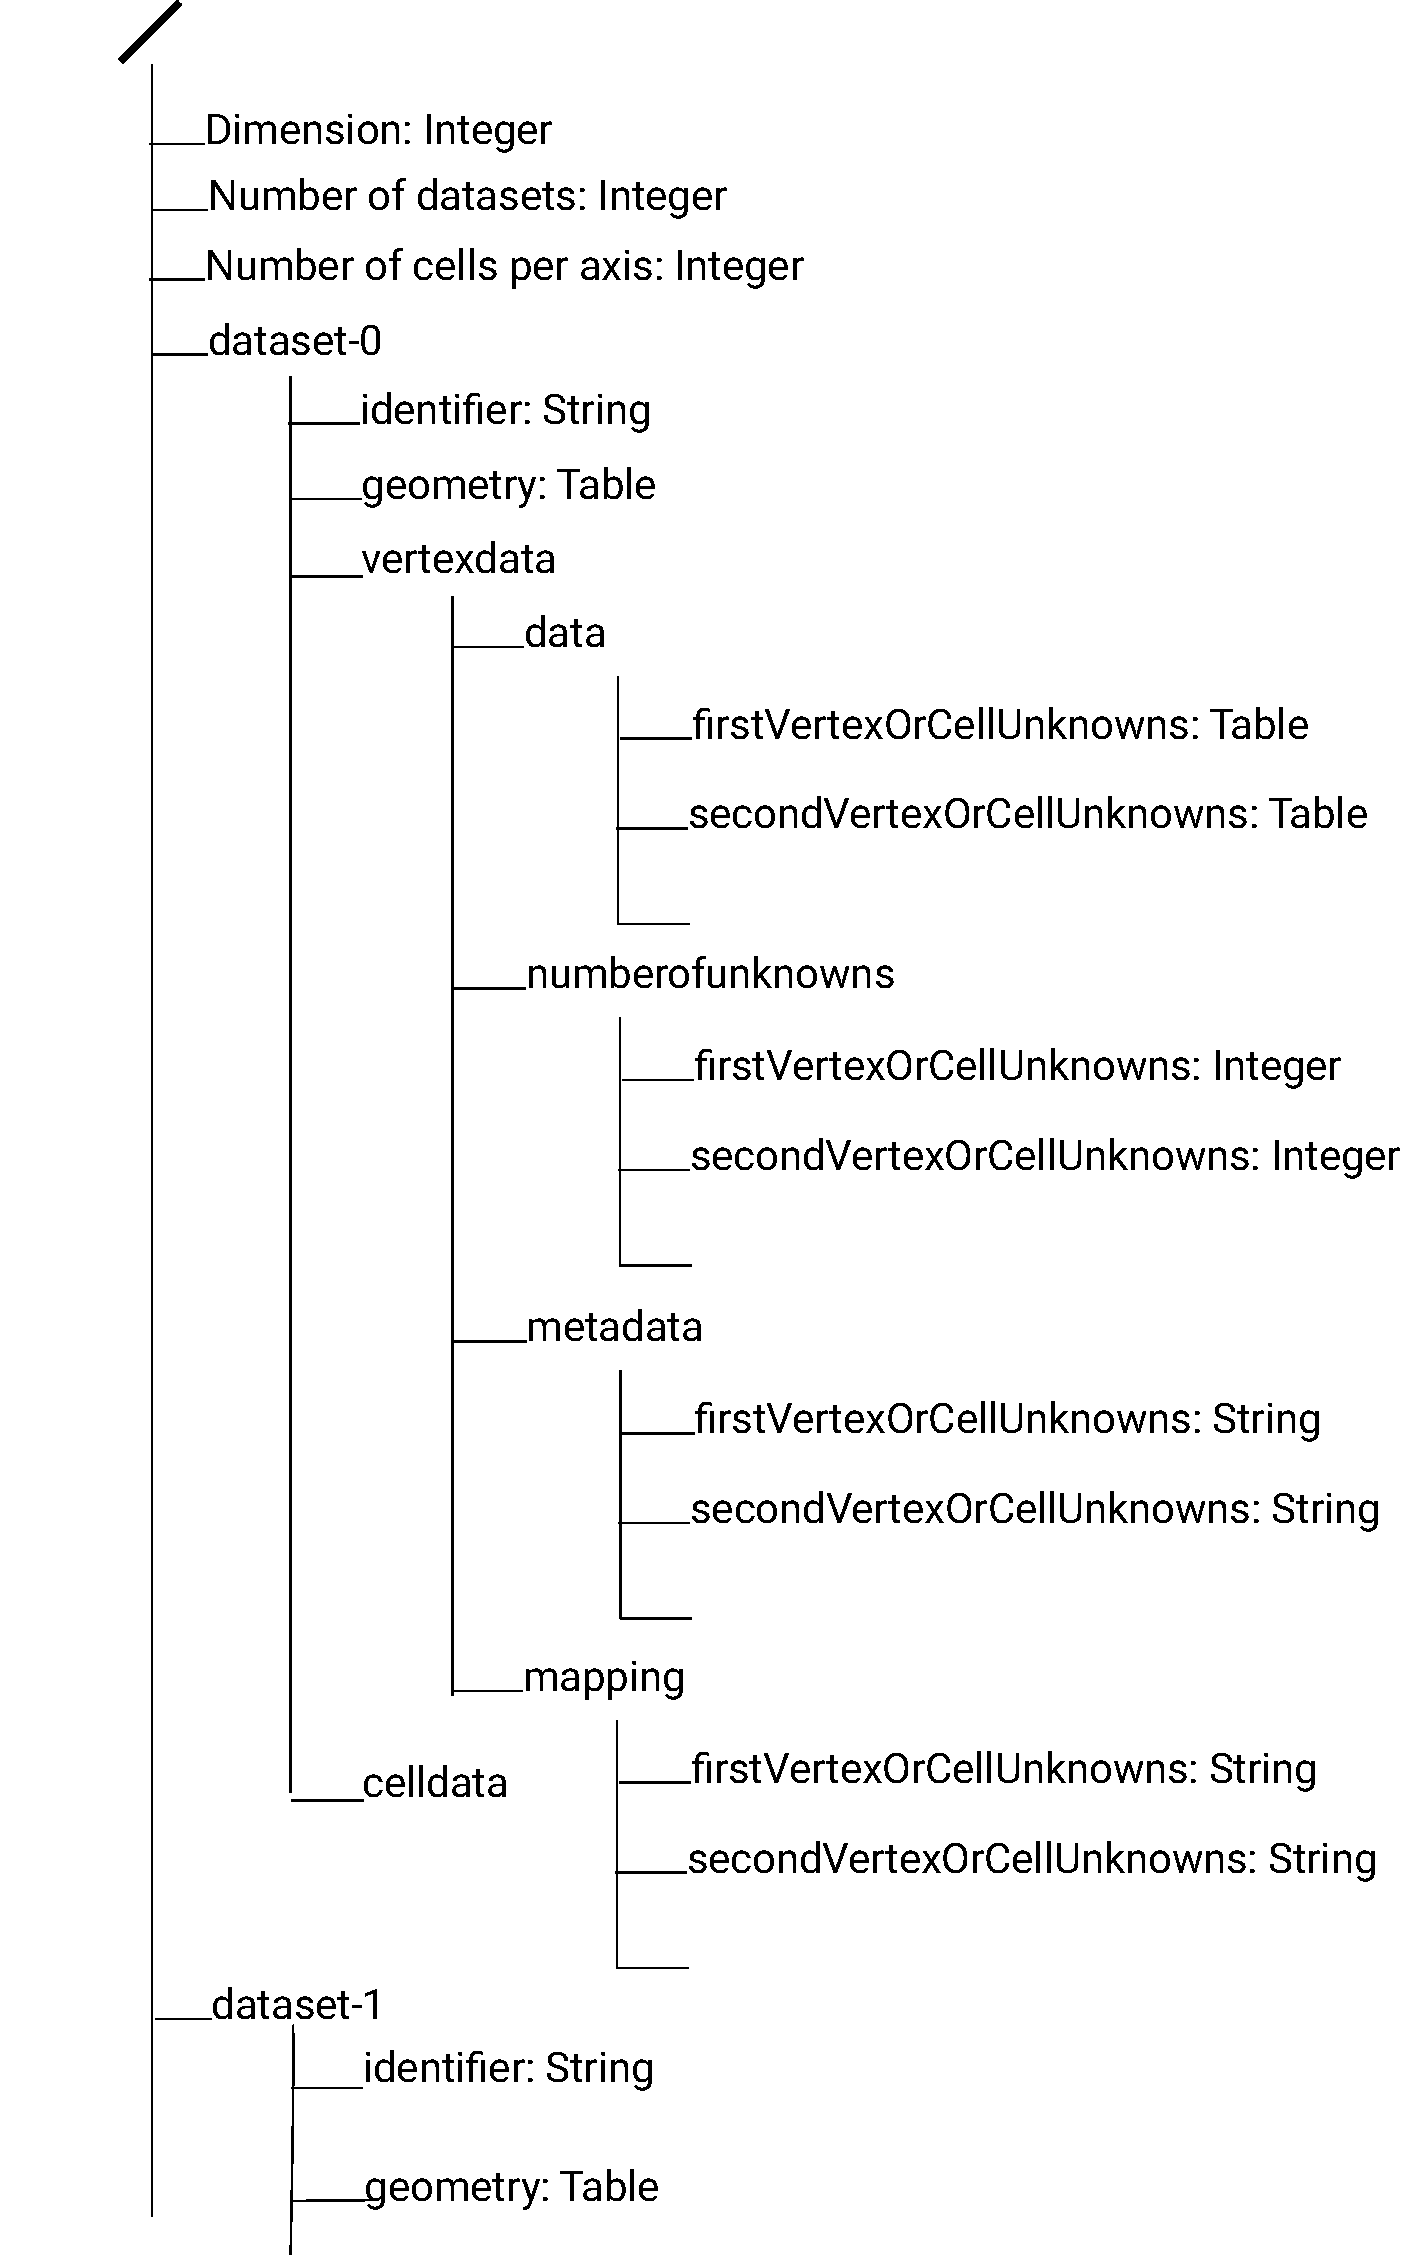
\includegraphics[width=0.4\textwidth]{81_blockstructured-file-format/hierarchy.pdf}
% \end{center}
% 
% \begin{itemize}
%   \item The root entry of the file holds an attribute \texttt{Number of
%   datasets} which is sole integer value.
%   \item For a given number of datasets, there are groups \texttt{dataset-x} with
%   \texttt{x} starting from 0.
%   \item The HDF5 root attribute \texttt{Dimensions} either holds 2 or 3.
%   \item Another HDF5 root attribute is \texttt{Number of cells per axis}. The
%   HDF dumps are basically unordered sequences of spacetree cells. Each cell can
%   be subdivided further into patches. In the trivial case, the patches are $1
%   \times 1 \times 1$ patches, i.e.~represent only cells. However they also can
%   be bigger.
%   \item Each group has an attribute \texttt{identifier} which stores a string.
%   If you use the native text or binary file formats of Peano, each snapshot
%   typically goes into a file of its own. For VTK, we then provide meta data
%   (through \texttt{VTKTimeSeriesWriter}) that summarises what the different
%   snapshots are called. The name is the argument you pass to
%   \texttt{writeToFile}. With HDF5, we consider the HDF file to be one container
%   that holds all these snapshots/subfiles, so the \texttt{identifier} holds
%   this argument from \texttt{writeToFile}.
%   \item Each dataset holds a table \texttt{geometry}. This table contains
%   one row per cell in the spacetree and the columns represent the offset and the sizes
%   of the cell.
%     \begin{center}
%       \begin{tabular}{l|ccc|ccc}
%         cell & $offset_x$ & $offset_y$ & $offset_z$ & $width_x$ & $width_y$ &
%         $width_z$ \\ 
%         \hline
%         0 & \ldots & \ldots & \ldots & \ldots & \ldots & \ldots \\
%         1 & \ldots & \ldots & \ldots & \ldots & \ldots & \ldots \\
%         2 & \ldots & \ldots & \ldots & \ldots & \ldots & \ldots \\
%       \end{tabular}
%     \end{center}
%   Obviously, there are either four or six entries per row. It depends on the
%   value held in \texttt{Dimensions}.
%   \item Each dataset holds two subfolders. One for data associated to vertices
%   and one for data associated to cells.
% \end{itemize}
% 
% 
% \noindent
% Users create per unknown that they want to pipe into the output file a vertex or
% cell writer. 
% They end up in the respective subfolders.
% Per written dataset, data ends up in up to four further subfolders:
% \begin{enumerate}
%   \item An entry in \texttt{mapping} is optional. If it is present, it holds a
%   table with \texttt{Dimensions} columns and $(\mbox{Number of
%   cells per axis})^{\mbox{Dimensions}}$ (if cell-based data) or  $(\mbox{Number
%   of cells per axis}+1)^{\mbox{Dimensions}}$ (if vertex-based data) rows.
%   They describe how the cell centres or vertices are distributed within a unit
%   cell or square. If you plot for example Gauss-Legendre points for an unknown,
%   this table encodes the positions of these points.
%   \item An entry in \texttt{metadata} is optional. If it is present, it contains
%   a string the describes the data.
%   \item The integer entry in \texttt{numberofunknowns} is mandatory. It
%   describes how many doubles are associated to each of the points within one
%   cell. If you study cell-based data with an entry of 1 here, then you simple
%   plot one scalar double per cell. If you embed $10^d$ patches into each cell
%   and if you plot vertex-based data, a 4 here implies that a user will find
%   $11^d \cdot 4$ doubles per cell data entry.
%   \item The table stored within \texttt{data} finally holds the actual
%   quantities. There is one table row per cell, i.e.~the number of rows equals
%   the number of rows in the \texttt{geometry} table. The number of columns
%   results from the description from the previous bullet point.
% \end{enumerate}
% 
% 
% \begin{remark}
%  Peano's blockstructured HDF5 format notably pays off if you embed whole patches
%  into the spacetree cells. If you use a low-order scheme with only one or two
%  doubles per cell, it does not pay off that much. The realisation also
%  implements on-the-fly compression (zip) through the plotter's constructor. This
%  way, you can bring down the required memory massively. 
% \end{remark}
